\chapter{Piattaforma di Simulazione}\label{chap:sim}

La piattaforma di simulazione è uno strumento di fondamentale importanza al fine di validare l'infrastruttura software proposta. Risulta inoltre essere un valido strumento per valutare l'impatto dell'introduzione della mobilità elettrica veicolare all'interno di un determinato contesto, grazie ad esso si può prevedere quanti veicoli sarà in grado di supportare la grid, quante colonnine saranno necessarie e che potenza dovranno avere. Risulta quindi uno strumento fondamentale sia sotto il punto di vista dell'amministrazione pubblica/cittadina, che può prevedere un piano urbanistico sostenibile, sia dal punto di vista dei gestori della rete elettrica, i quali potranno valutare la richiesta energetica di tale scenario ed eventualmente prevedere investimenti in quella direzione.

\section{Architettura}

Al fine di poter simulare gli innumerevoli aspetti legati all'Electrical Mobility sono stati usati diversi simulatori/tecnologie in simbiosi. In questa sezione verranno introdotte brevemente al fine di introdurre al resto della trattazione.

\subsection{SUMO}\label{sebsec:sumo}

SUMO (Simulator of Urban Mobility) è un simulatore Open Source e multi-piattaforma di traffico urbano progettato per simulare reti stradali di grandi dimensioni. Sviluppato in C++ è supportato principalmente dall'Institute of Transportation Systems at the German Aerospace Center. La simulazione è di tipo microscopico ovvero ogni veicolo è modellato in modo esplicito, ha un proprio itinerario e si muove individualmente attraverso la rete. Ogni aspetto relativo alla simulazione viene configurato attraverso file XML i quali descrivono la rete stradale, i parametri ed i percorsi di ogni singolo veicolo, ed eventualmente altri aspetti legati alla simulazione come i flussi di traffico oppure la descrizione degli edifici. 

SUMO permette di avviare la simulazione in due modalità:

\begin{itemize}
	\item \textbf{Visuale}: La modalità visuale permette di avere un riscontro visuale l'andamento della simulazione tramite un interfaccia che mostra la mappa della rete/città con vista dall'alto. Vengono mostrati tutti i veicoli ed è possibile accedere a tutti i parametri della simulazione. Vengono mostrati inoltre i semafori agli incroci, la segnaletica delle strade e, nel caso siano stati caricati, gli edifici della città. Tutto questo ovviamente impatta notevolmente sulle performance ma, al di la del gradevole effetto visivo, è utile per vedere come evolve la simulazione. Nel nostro caso, ad esempio, è servito per assicurarsi che i veicoli si fermassero alle colonnine, oppure per valutare la quantità di traffico generata in seguito all'inserimento di un determinato numero di veicoli. Molto utile è stato anche in fase di Demo per mostrare il funzionamento del nostro simulatore.
	\item \textbf{Testuale}: Con la modalità testuale vengono stampati nel terminale i messaggi di Warning ed Error nel terminale e se richiesto anche qualche messaggio di debug in più che indica gli step di avanzamento della simulazione. Dopo aver constatato che la simulazione si comporta come ci si aspetta tramite la modalità visuale si passa allora a questa modalità che ha performance assai maggiori. È quindi particolarmente indicata per le simulazioni di lunga durata.
\end{itemize}

\subsubsection{Tools}\label{sumo-tools}

I file XML che descrivono le simulazioni possono diventare molto complessi qualora si decida di simulare scenari realistici (come Bologna). SUMO mette a disposizione innumerevoli tool automatici per la generazione dei file di configurazione.  In questa tesi prenderemo in esame solo quelli che ci sono stati utili:

\begin{itemize}
 	\item \textbf{netconvert}: Genera file con estensione .net.xml della dove viene mappata la rete stradale. La generazione avviene in modo pseudo-casuale, tramite la definizione dei nodi e degli archi che definiscono il "grafo" della rete stradale oppure, come nel nostro caso, attraverso la conversione da formati esterni(OpenStreetMap, VISUM, VISSIM, OpenDRIVE, MATsim ecc..)
 	\item \textbf{polyconvert}: Genera file con estensione .poly.xml dove sono contenute le informazioni relative agli edifici, zone di verde, fiumi laghi ecc.. Anch'esse vengono importate dai file delle mappe in altri formati.
 	 \item \textbf{duarouter}: Genera file con estensione .rou.xml che descrivono per ogni veicolo il suo percorso, compresi tutti i suoi step intermedi. La generazione dei percorsi avviene applicando un algoritmo di cammino su grafi a scelta tra Dijikstra o A*. I punti di partenza e arrivo vengono generati casualmente da uno script in python messo a disposizione tra i tool di sumo (randomTrips.py).
\end{itemize}

\subsubsection{TRaCI}

TraCI (Traffic Controller Interface) è un modulo messo a disposizione da SUMO che permette di interagire con la simulazione in tempo reale tramite un protocollo Client/Server basato su TCP/IP. All'avvio della simulazione SUMO si mette in ascolto su una porta in attesa di messaggi, qualunque linguaggio che supporti il protocollo TCP/IP può dunque modificare lo stato della simulazione oppure ricevere notifiche sul cambiamento di variabili alle quali ci si può sottoscrivere. È proprio TraCI che farà da ponte tra SUMO e l'altro simulatore usato all'interno della nostra piattaforma.

\subsection{OMNeT++}
OMNeT++ è un ambiente OpenSource di simulazione a eventi discreti. È principalmente usato per la simulazione di reti di comunicazione, ma grazie alla sua architettura modulare ed estremamente flessibile è possibile utilizzarlo negli ambiti più disparati come la simulazione di sistemi informatici complessi, architetture hardware o, come nel nostro caso, per supporto alla simulazione veicolare.

Le simulazioni vengono modellate tramite l'impiego di componenti riusabili chiamati \emph{moduli} i quali possono essere combinati tra loro come dei blocchi LEGO.

I moduli possono essere connessi tra di loro attraverso i \emph{gates} e combinati insieme per formare dei moduli composti (compound modules). La comunicazione tra moduli normalmente avviene tramite message passing e i messaggi possono contenere strutture dati arbitrarie (a parte informazioni predefinite tipo i timestamp). Questi messaggi possono viaggiare attraverso percorsi predefiniti dai gates e dalle connections oppure essere inviati direttamente alla loro destinazione, quest'ultima scelta è molto utile nel caso delle comunicazioni wireless. 

I moduli, i relativi parametri e i collegamenti fra loro, vengono definiti tramite un linguaggio di alto livello (NED) in appositi file con estensione .ned, mentre la logica viene implementata in una corrispondente classe C++.

OMNeT++ viene distribuito con un IDE basato su Eclipse grazie al quale possono essere eseguite molte operazioni in modo visuale, come ad esempio la creazione e aggregazione di moduli.

Anche OMNeT++ mette a disposizione due modalità di esecuzione della simulazione una visuale (\emph{Tkenv}) e una testuale (\emph{Cmdenv}). La modalità visuale permette di vedere i moduli con i relativi messaggi che vengono scambiati, viene usata in fase di debug o in fase di Demo. La modalità testuale, ovviamente più performante e adatta alle simulazioni batch, mostra solo i messaggi di debug della simulazione insieme allo standard output dei moduli. Per i nostri scopi abbiamo usato solo la modalità testuale.

Un grande punto di forza di OMNeT++ sono gli strumenti messi a disposizione per l'analisi dei dati generati dalle simulazioni, che permettono di applicare, in tempo reale, trasformazioni e aggregazioni tra i set di dati e, in fine, visualizzare i risultati con varie tipologie di grafici: a barre, a linee, istogrammi e molti altri.

Ci sono due tipi di dato che si possono registrare in OMNeT++ i vettori e gli scalari, ne caso dei vettori si hanno i dati sul piano cartesiano, con il tempo come ascissa e il dato come ordinata, mentre nel caso degli scalari viene registrato un solamente un dato.

\subsection{Veins}\label{subsec:veins}

Veins è un framework OpenSource per la simulazione di reti veicolari IVC (Inter-Vehicular Communication). Utilizza OMNeT++ e SUMO in simbiosi. Si appoggia su MiXiM, un framework per OMNeT++, che implementa modelli per reti wireless fisse e mobili (reti di sensori wireless, reti ad hoc, reti veicolari ecc.). La comunicazione con SUMO avviene tramite TRaCI. Ogni volta che nella simulazione in SUMO viene aggiunto un veicolo Veins crea dinamicamente un corrispondente modulo OMNeT++ che permette di controllarlo sotto ogni aspetto (percorso, colore, velocità, accelerazione, parcheggio ecc..).

Il simulatore consiste in un modulo di Veins, il quale è stato opportunamente modificato al fine di avere un ambiente che contiene solo i componenti strettamente necessari allo scopo in quanto le performance sono determinanti al fine di poter avere dei risultati in tempi utili. Infatti sono stati rimossi da Veins i moduli necessari alla comunicazione wireless (nic80211 e ARP), il modulo per la gestione degli ostacoli (obstacles) che era utilizzato per la gestione dello shadowing delle reti wireless

\subsubsection{Il funzionamento di Veins}\label{subsubsec:veins-func}

Veins è il ponte tra OMNeT++ e SUMO e la comunicazione tra i due avviene tramite TraCI. In realtà "in mezzo" ai due simulatori si trova uno script python, \emph{sumo-launchd.py}, che sta in ascolto sulla prima porta libera che trova, in attesa che venga avviato Veins. Quando Veins viene avviato si connette a questo script il quale lancia SUMO, a questo punto inizia la sincronizzazione tra i due simulatori che avviene tramite "staffetta" come mostrato in Fig. ~\ref{fig:veins-state-machine}. Per garantire l'esecuzione sincrona a intervalli definiti Veins inserisce in un buffer tutti i comandi da inviare a SUMO (Fig.  ~\ref{fig:veins-sequence-diagram}). Ad ogni passo temporale, i comandi contenuti nel buffer vengono inviati. Ciò innesca l'avanzamento del corrispondente passo temporale nella simulazione del traffico stradale. Al termine dello step temporale di simulazione del traffico stradale, SUMO invia una serie di comandi con lo stato e la posizione di tutti i veicoli istanziati in risposta a Veins. Dopo l'elaborazione di tutti i comandi ricevuti Veins aggiunge i corrispettivi nodi per ogni nuovo veicolo introdotto nella simulazione e rimuove invece i nodi relativi ai veicoli che sono giunti a destinazione. A questo punto la simulazione può avanzare al prossimo step temporale.

\begin{figure}[H]
        \centering
        \begin{subfigure}[H]{0.5\textwidth}
                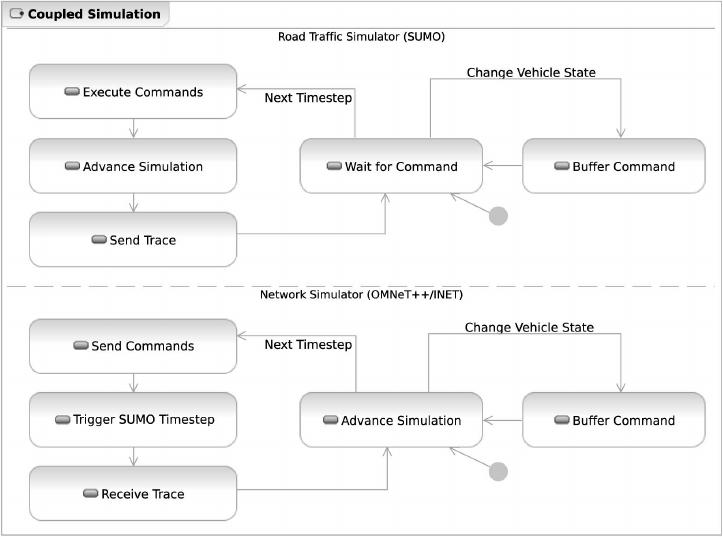
\includegraphics[width=\textwidth]{assets/veins-state-machine.jpg}
                \caption{Panoramica dei due simulatori abbinati. Macchina a stati di SUMO e i moduli di Veins.}
                \label{fig:veins-state-machine}
        \end{subfigure}%
        ~ %add desired spacing between images, e. g. ~, \quad, \qquad etc.
          %(or a blank line to force the subfigure onto a new line)
        \begin{subfigure}[H]{0.5\textwidth}
                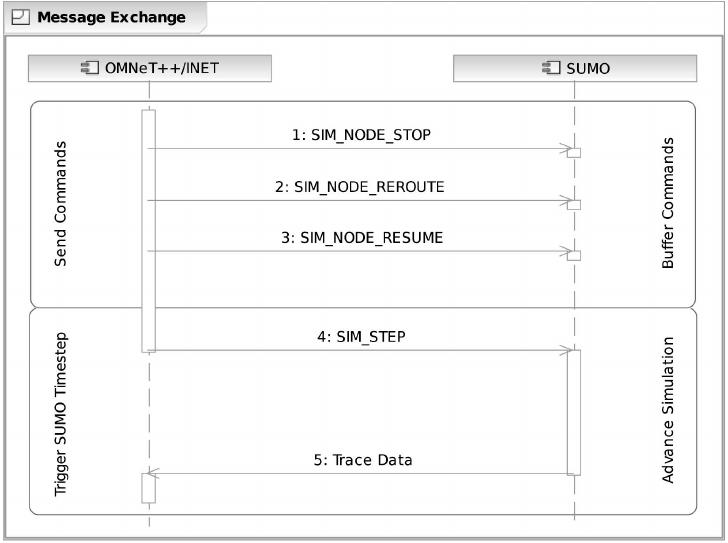
\includegraphics[width=\textwidth]{assets/veins-sequence-diagram.jpg}
                \caption{ Diagramma di sequenza dei messaggi scambiati tra SUMO e Veins. L'esecuzione dei comandi è ritardata fino al successivo passo temporale in SUMO.}
                \label{fig:veins-sequence-diagram}
        \end{subfigure}
        \caption{Architettura Veins}
\end{figure}


\section{Modellazione della Simulazione}

L'intera simulazione viene incapsulata all'interno di una Network. Il Network è lo scenario da simulare, all'interno di esso si definiscono i moduli che compongono la simulazione. Come mostrato in Fig \ref{fig:module-scenario} sono sostanzialmente 4 i moduli che compongono la nostra simulazione:

\begin{itemize}
	\item \textbf{world}: È un modulo di tipo \code{BaseWorldUtility}, fornito da MiXiM, che rappresenta l'area che circoscrive lo scenario simulato. Come configurazione richiede di definire la grandezza dello scenario in metri. La mappa usata in SUMO non può essere più grande delle dimensioni definite in questo modulo.
	\item \textbf{manager}: È un modulo di tipo \code{TraCIScenarioManagerLaunchd}, fornito da Veins, che mette in comunicazione OMNeT++ con SUMO. Tutte i messaggi inviati a TraCI passano da questo modulo (l'implementazione vera e propria della comunicazione con TraCI avviene nel modulo padre \code{TraCIScenarioManager}). Questo modulo è fondamentale in quanto è quello che crea un modulo OMNeT++ per ogni veicolo di SUMO.
	\item \textbf{cityService}: Rappresenta la grid, infatti contiene i GCP e gli EVSE. Ricopre anche la funzione di raccoglitore statistiche globali sulle colonnine e i veicoli (Sez: \ref{sec:module-city}).
	\item \textbf{connectionManager}: Questo modulo si occupa della comunicazione tra moduli ma è inutilizzato. Non l'ho rimosso per questioni di compatibilità con Veins.
\end{itemize}

Ogni volta che SUMO crea un veicolo Veins si occupa di creare il corrispondente modulo in OMNeT++, il modulo in questione è Car (Fig. \ref{fig:module-car}). Car in realtà è un modulo composto ovvero un contenitore, privo di implementazione, che contiene altri moduli. Di default, conterrebbe tutti i componenti relativi alle comunicazioni wireless in quanto sarebbe il target di Veins, ma io li ho rimossi in quanto non utili, per ora, nel nostro scenario.

Al fine di rendere la simulazione il più possibile attinente alla realtà risulta necessario implementare i modelli di carica e scarica dei veicoli e i modelli comportamentali degli utenti nonché l'implementazione dei moduli di comunicazione con il servizio cittadino. Per svolgere questi compiti è stato necessario arricchire la definizione di Car con 3 nuovi moduli:

\begin{itemize}
	\item \textbf{TraciMobility}: È un modulo fornito da Veins che mette in comunicazione il veicolo con OMNeT++ tramite TRacI.
	\item \textbf{CarLogic}: È il modulo principale, in esso è implementata la logica del veicolo. 
	\item \textbf{Battery}: Implementa il modello di carica e scarica del veicolo.
	\item \textbf{DriverBehaviour}: In questo modulo sono implementati i comportamenti che l'utente assume dinanzi a determinate scelte.  
\end{itemize}

Ogni modulo contiene dei parametri che permettono di cambiarne il comportamento, grazie a OMNeT++ diventa semplice lanciare molteplici simulazioni con diversi set di dati. Particolarmente interessante è la possibilità di eseguire la simulazione senza prenotazione per poter confrontare le differenze di occupazione delle colonnine rispetto allo scenario con prenotazione.

\begin{figure}[H]
        \centering
		\begin{subfigure}[H]{0.45\textwidth}
                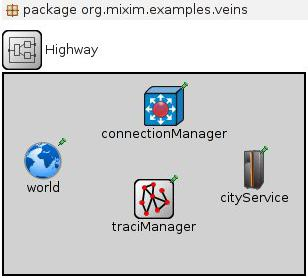
\includegraphics[width=\textwidth]{assets/module-scenario.jpg}
                \caption{Modulo scenario}
                \label{fig:module-car}
        \end{subfigure}
        \qquad
        \begin{subfigure}[H]{0.45\textwidth}
                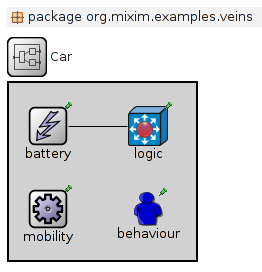
\includegraphics[width=\textwidth]{assets/module-car.png}
                \caption{Modulo Car}
                \label{fig:module-scenario}
        \end{subfigure}%
        \caption{Moduli OMNeT++}
\end{figure}

\subsection{Ciclo di Vita dei moduli}\label{subsec:lifecycle}

Essendo OMNeT++ un simulatore a eventi discreti i moduli, in esso implementati, non fanno nulla finché non viene schedulato un evento. Gli eventi vengono schedulati attraverso messaggi inviati dai moduli stessi. Sostanzialmente si tratta di decidere quando, a chi e cosa mandare.
Il quando è il tempo di simulazione e quindi deve essere nel futuro o al massimo nel momento attuale di simulazione, a chi è il modulo destinatario e cosa è il messaggio da mandare. OMNeT++ fornisce un un messaggio di base, \code{cSimpleMessage}, ma, come vedremo più avanti, è possibile definirsi messaggi propri più complessi.

All'interno di questa simulazione non avviene molto scambio di messaggi tra i diversi moduli, ragion per cui risulta necessario auto-inviarsi i messaggi al fine di mantenere "vivo" il modulo.

Quando Veins crea un modulo il corrispondente veicolo in SUMO viene aggiornato ogni 0.1 secondi, che è lo step temporale di default. In OMNeT++ invece siamo noi a decidere ogni quanto aggiornare un modulo attraverso il meccanismo degli auto-messaggi. Schedulando i messaggi in modo intelligente si può guadagnare in performance in quanto ci si può inviare il messaggio solo quando è realmente necessario.

Quando un modulo Car viene creato viene chiamata la funzione \code{initialize()}, della quale il programmatore può eseguire l'override, nella quale dopo le opportune inizializzazioni, è necessario auto-schedularsi un messaggio. I messaggi vengono ricevuti dalla funzione \code{handleMessage()} alla quale viene passato un riferimento al messaggio stesso. Da dentro questa funzione si può implementare la logica del modulo. Il modulo continua a vivere finché, il corrispondente veicolo in SUMO, non giunge a destinazione momento in cui Veins, attraverso la classe \code{TraCIScenarioManager}, si accorge che il veicolo non è più nella simulazione e quindi lo elimina anche da OMNeT++ il che causa una chiamata alla funzione di terminazione \code{finish()}.

\subsection{CityService}\label{sec:module-city}

Il modulo CityService simula la grid, al suo avvio carica le informazioni relative ai GCP presenti nello scenario simulato da un file XML. Il file utilizzato è lo stesso del servizio cittadino (Sez. ~\ref{subsubsec:city-init}). Le colonnine caricate vengono trasformate in oggetti C++ al fine di poter essere usate dai veicoli virtuali. 

Questo modulo, attraverso il settaggio di parametri esterni, provvede ad abilitare/disabilitare le prenotazioni, e inoltre decide il tasso di penetrazione di veicoli elettrici nello scenario.

Quelli mostrati di seguito sono i parametri del modulo:

\begin{itemize}
	\item \code{gcpList}: Percorso del file XML che contiene la definizione dei GCP. Deve essere lo stesso utilizzato dal servizio cittadino reale.
	\item \code{electricalVehicleFreq}: Questo parametro stabilisce la frequenza con cui viene immesso un veicolo elettrico nella simulazione. È un numero che può variare da 0 a 100 e, più precisamente, indica con quale probabilità il veicolo inserito nella simulazione è elettrico. È necessario ricordare che il numero e la frequenza con cui i veicoli vengono immessi nella simulazione è determinato da SUMO attraverso i suoi file di configurazione. 
	\item \code{maxElectricalVeh}: Impone un limite superiore al numero di veicoli che possono essere presenti nella simulazione in un determinato istante. Questo significa che se è stato raggiunto il massimo numero di veicoli, e uno di questi lascia la simulazione per un qualunque motivo, allora verrà rimpiazzato da uno nuovo (sempre ammesso che SUMO generi altri veicoli e che la statistica sia favorevole). Se viene impostato a -1 allora non ci sarà nessun limite al numero di veicoli.
	\item \code{reservationEnabled}: Abilita/Disabilita il protocollo di prenotazione per i veicoli. l fine di ottimizzare le performance lo scambio di dati con il SIB, necessario per le prenotazioni, viene completamente disabilitato quando quest'ultime non sono attive.
\end{itemize}

Altra importante funzione svolta da questo modulo è la raccolta di statistiche globali sui veicoli elettrici. I dati raccolti sono tutti in formato vettoriale:

\begin{itemize}
	\item \textbf{chargingVehicles}: In questo vettore viene salvato lo stato di occupazione degli EVSE della città, ogni volta che un veicolo si va a ricaricare aggiunge un unità al vettore e quando finisce la ricarica l'unità viene rimossa. Questo comporta che come ordinata avremo al massimo il numero totale di EVSE presenti nello scenario.
	\item \textbf{electricalVehicles}: Numero di veicoli elettrici presenti nella simulazione, semplicemente ogni volta che viene aggiunto un veicolo elettrico alla simulazione viene incrementata di un unità il vettore.
	\item \textbf{vaporizedVehicles}: I veicoli vaporizzati sono quei veicoli che hanno terminato la batteria e quindi vengono letteralmente vaporizzati. Il termine vaporizzati deriva dall'analogo comando di TRacI che permette di rimuovere un veicolo dalla simulazione. 
	\item \textbf{leavingVehicles}: Questo veicolo tiene traccia dei veicoli che riescono a lasciare normalmente la simulazione ovvero arrivano a destinazione, evento che ne causa la rimozione da parte di SUMO. In realtà uno degli obbiettivi raggiunti è stato proprio quello di dirottare i veicoli che arrivano a destinazione verso una strada casuale. Non è sempre possibile intercettare l'arrivo del veicolo in una determinata strada, questo comporta che qualcuno di essi "sfugga" e venga rimosso dalla simulazione.
\end{itemize}


\subsection{CarLogic}

Il comportamento del veicolo è definito dal modulo CarLogic. Questo modulo implementa tutta la logica relativa alla guida del veicolo. In esso sono contenute le informazioni che ne descrivono la tipologia, l'appartenenza, e alcuni comportamenti di base. I comportamenti più complessi sono delegati al modulo DriverBehviour.

\begin{itemize}
	\item \code{userName}: Nome dell'utente che possiede il veicolo
	\item \code{userId}: Identificativo dell'utente che possiede il veicolo
	\item \code{manufacturer}: Casa produttrice del veicolo
	\item \code{model}: Modello del veicolo
	\item \code{cRoll}: Resistenza attrito gomme su asfalto
	\item \code{cDrag}: 
	\item \code{across}: Sezione frontale del veicolo
	\item \code{rhoAir}: Resistenza dell'aria
	\item \code{weight}: Peso del veicolo
	\item \code{threshold}: Soglia sotto la quale il veicolo si considera scarico e quindi diviene necessario fare una ricarica. Varia da 0 a 1.
	\item \textbf{minRequestedEnergyKwh}: Quantità minima di energia richiedibile in una richiesta di prenotazione. Questo valore serve nei casi in cui una richiesta non venga accettata dal \emph{City Service}, in tal caso viene diminuita gradualmente la quantità di energia richiesta fino ad arrivare a questa soglia.
	\item \textbf{writeCarStatusOnSib}: Dice se scrivere le informazioni di stato dei veicoli sul \emph{Dash SIB}. Questo permette di vedere lo stato dei veicoli dall'applicazione mobile. Essendo la scrittura sul SIB un operazione abbastanza onerosa è meglio tenere disattivata questa opzione a meno che non si sia in fase di demo.
\end{itemize}


\subsubsection{Inizializzazione}

In fase di inizializzazione la prima cosa che viene fatta è prendere un riferimento a tutti i moduli necessari, tra i quali il CityService, che  deciderà se il veicolo sarà elettrico o meno. Nel caso in cui sia elettrico allora si procede a reperire tutti i parametri e, se è abilitata la prenotazione, vengono scritte le informazioni del veicolo sul \emph{Dash SIB}. Viene inoltre mandato un comando a SUMO colora il veicolo di verde, funzionalità molto utile sia in fase di debug che in fase di demo.

Nel caso in cui il veicolo non sia elettrico allora vengono eliminati i relativi moduli da OMNeT++ ma il veicolo rimane in SUMO. Questa funzionalità non era prevista da Veins e quindi è stato necessario modificarlo opportunamente per introdurla. L'eliminazione avviene indirettamente, dal momento che un modulo di Veins non può eliminare se stesso, mandando un messaggio al CityService con la richiesta di eliminazione.

Un problema di SUMO, almeno per quelli che sono i nostri obbiettivi, è che un veicolo una volta giunto alla sua destinazione viene eliminato dalla simulazione. Questo comportamento influisce negativamente sulla simulazione in quanto a noi interessa simulare un periodo di vita dei veicoli lungo abbastanza da poterne studiare diversi cicli di carica e scarica. Per sopperire a questo problema vengono ottenuti, tramite TraCI, gli ID di tutte le strade che compongono il percorso del veicolo e viene preso l'ultimo in modo da poter intercettare l'arrivo del a quest'ultimo e quindi dirottarlo verso un'altra destinazione casuale. Le altre destinazioni vengono scelte da una lista che viene riempita con gli ID elle strade di destinazione, prese dai veicoli stessi, più lunghe di 50 metri. Il controllo sulla lunghezza serve in quanto è più probabile intercettare il momento in cui il veicolo arriva  a destinazione.

A questo punto come ultima operazione viene istanziato un messaggio di tipo \code{CarMessage}, appositamente creato per mantenere lo stato del veicolo attraverso le varie transazioni di stato. I campi del messaggio vengono inizializzati e il messaggio viene schedulato al tempo attuale di simulazione. Come si vede nel List. \ref{lst:omnet-msg} il messaggio viene creato, viene impostato lo stato del veicolo (Sez. \ref{subsubsec:veh-state}), e infine viene schedulato tramite la funzione \code{scheduleAt()} al tempo attuale di simulazione che viene fornito dalla funzione \code{simTime()}. Per schedulare il messaggio dopo 25 secondi sarebbe stato necessario usare \code{simTime() + 25}.

\begin{cpp}[caption={Autoschedulazione Messaggio},label={lst:omnet-msg}]
carMessage = new CarMessage("CarMessage");
carMessage->setCarState(CarState::DRIVING);
[...]
scheduleAt(simTime(), carMessage);
\end{cpp}


\subsubsection{Gli stati del veicolo}\label{subsubsec:veh-state}

Lo stato del veicolo è definito da un automa a stati finiti come mostrato in Fig. \ref{fig:car-fsmd}. Le transazioni tra gli stati avvengono tramite scambio di messaggi nei quali è definito lo stato successivo. I messaggi arrivano alla funzione \code{handleMessage} la quale controlla se il messaggio arriva dall'esterno oppure se è auto-inviato (\code{msg->isSelfMessage()}). In quest'ultimo caso allora il messaggio viene inoltrato a una funzione chiamata \code{handleSelfMessage()}. All'interno di quest'ultima funzione avviene la scelta di quale hanlder eseguire in base allo stato definito nel messaggio (Lst. \ref{lst:self-msg}).

\begin{cpp}[caption={Funzione di scelta dello stato}, label={lst:self-msg}]
void CarLogic::handleSelfMessage(cMessage *msg) {
	CarMessage* carMsg = check_and_cast<CarMessage *>(msg);
	
	switch (carMsg->getCarState()) {
		case CarState::DRIVING:
			handleDriving(carMsg);
			break;
		[...]
		case CarState::CHARGING:
			handleCharging(carMsg);
			break;
		default:
			error("Unknown Car State!");
			break;
	}	
}
\end{cpp}

Ogni stato del veicolo ha una sua funzione "handler" che ne determina il comportamento. Alla funzione viene passato un riferimento al messaggio che contiene informazioni sullo stato del veicolo. L'handler prima di finire rischedula il messaggio con un nuovo stato, o con lo stesso in alcuni casi. La Fig. \ref{fig:car-fsmd} mostra l'automa a stati finiti che descrive il veicolo. 

I possibili stati del veicolo sono definiti nell'enumerazione \code{CarState}. Sarà quindi presente, ad esempio, la funzione \code{handleDriving} associata allo stato \code{CarState::DRIVING}, e così via per tutti gli stati del veicolo.

Dal momento che l'implementazione C delle KPI, le librerie che si interfacciano con il SIB tramite il protocollo SSAP (Sez. \ref{sec:smart-m3}), non supporta le sottoscrizioni, che sono alla base della comunicazione con il CS, risulta necessario fare il ``polling'' a intervalli regolare per ricavare le risposte. A questo compito sono stati riservati due stati del veicolo \code{WAITING_RESPONSE} e \code{WAITING_CONFIRM}. 

\begin{description}
	\item \label{state:driving} \code{DRIVING}: Quando il veicolo si trova in questo stato significa che si sta dirigendo verso la sua destinazione. Ogni volta che viene eseguito fa un controllo sullo stato di carica della batteria e se questa è inferiore alla soglia stabilita dal parametro \code{threshold} allora il veicolo si considera scarico e quindi riuslta necessario dirigesi a una colonnina. A questo punto si presentano due casistiche:
	\begin{itemize}
		\item{Con Prenotazione}: se la simulazione è stata eseguita con le prenotazioni attive allora il veicolo deve eseguire il protocollo di prenotazione. Vengono quindi create le triple necessarie a istanziare una richiesta di prenotazione e inserite nel SIB. Se la richiesta va a buon fine allora si imposta come stato successivo \code{WAITING_RESPONSE}, altrimenti viene rischedulato questo e reiterata la richiesta.
		\item{Senza Prenotazione}: Se la simulazione è stata eseguita senza prenotazione allora viene scelto casualmente un GCP tra i 3 più vicini e il veicolo dirige direttamente verso quello passando nello stato \code{GO_TO_RECHARGE}.
	\end{itemize}
	\item \code{WAITING_RESPONSE}: il veicolo interroga il SIB in cerca della risposta da parte del CS. La ricerca è eseguita tramite query SPARQL. Se fallisce, oppure restituisce un risultato vuoto (non sono disponibili opzioni di ricarica conformi alla richiesta), il veicolo torna in stato \code{DRIVING} dove la richiesta viene reiterata diminuendo l'energia richiesta e aumentando il lasso di tempo in cui si è disposti a caricarsi. Se la query restituisce una risposta allora vengono analizzate le opzioni di ricarica in essa contenute e, in base al comportamento definito in \code{DriverBehaviour}, ne viene scelta una. Lo stato successivo sarà  \code{WAITING_CONFIRM}
	\item \code{WAITING_CONFIRM}: il veicolo interroga il SIB in cerca della conferma da parte del CS. Analogamente a quanto succede nello stato precedente se la ricerca fallisce ho ha esito negativo si ritorna in stato \code{DRIVING}. In caso di successo è impostata come destinazione la strada del GCP dove avverrà la ricarica. Se il tempo che manca alla ricarica è maggiore di un quarto d'ora allora il veicolo passa in stato \code{PARKING} in attesa dell'orario della ricarica, questo comportamento serve ad evidenziare il fatto che un utente che dispone della prenotazione è meno ansioso rispetto a uno che invece deve girare tutti i GCP della città fino a che non trova un EVSE libero. Se il tempo che manca alla ricarica è minore di un quarto d'ora allora il veicolo si dirige verso al GCP passando in stato \code{GO_TO_RECHARGE}
	\item \code{PARKING}: il veicolo si parcheggia nella prima strada disponibile in attesa del tempo necessario alla ricarica. Lo stato successivo viene definito nello stato precedente a questo. Attualmente il solo stato che porta a \code{PARKING} è \code{WAITING_CONFIRM} e come stato successivo imposta \code{GO_TO_RECHARGE}.
	\item \code{GO_TO_RECHARGE}: il veicolo si dirige verso il GCP. Controlla periodicamente la strada in cui si trova e quando arriva in quella del GCP  si ferma. A questo punto si presentano due casistiche:
	\begin{itemize}
		\item{Con Prenotazione}: Se la colonnina è occupata allora il veicolo, che evidentemente è arrivato in anticipo, si mette in coda in attesa del suo turno passando nello stato \code{WAITING_FOR_EVSE} altrimenti inizia la ricarica e si passa in stato \code{CHARGING}.
		\item{Senza Prenotazione}: Si controlla se ci sono degli EVSE liberi e in tal caso inizia la ricarica passando in stato \code{CHARGING}. In assenza di EVSE allora si interroga il modulo \code{DriverBehaviour} che stabilisce se fermarsi ad aspettare il veicolo che si sta caricando attualmente passando nello stato \code{WAITING_FOR_EVSE}. In caso contrario si sceglie casualmente un GCP tra i tre più vicini che non siano già stati visitati e ci si dirige verso di esso passando nello stato \code{GO_TO_RECHARGE}. 
	\end{itemize}
	\item \code{WAITING_EVSE}: questo stato rappresenta l'attesa presso un EVSE. Non viene schedulato nessun messaggio poiché è compito del veicolo attualmente in carica ``risvegliare'' il veicolo in attesa. Lo stato successivo al ``risveglio'' è \code{CHARGING}
	\item \code{CHARGING}: Rappresenta la carica lo stato di carica di un veicolo. Si rimane in questo stato finché la carica non è completa oppure, nel caso di prenotazione attiva, fino al raggiungimento del tempo di fine ricarica.
\end{description}
	
\begin{figure}
	\centering
	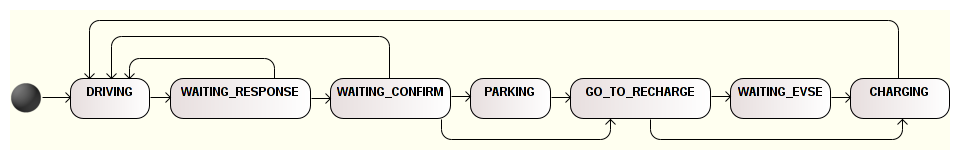
\includegraphics[width=1.0\textwidth]{assets/car-fsmd.png}
	\caption{Automa a stati finiti che descrive il veicolo, tutti gli stati possono essere finali.}
	\label{fig:car-fsmd}
\end{figure}

\subsection{Battery}\label{sec:battery}

\subsection{DriverBeahviour}

\section{Implementazione}

????
Esisteva già una versione del simulatore ma era a puro titolo dimostrativo e di demo e soffriva del fatto che era stato sviluppato da diverse persone (me compreso) in tempi molto brevi e con deadline che corrispondendo a demo internazionali si era costretti a rispettare. Questo ha portato ad avere un codice farraginoso e pieno di memory leak. Basti pensare che la prima versione del simulatore allocava RAM esponenzialmente e già dopo 2000 secondi si poteva arrivare ad avere un occupazione di 4GB.

La prima cosa che ho fatto, quando ho capito che la situazione stava diventando ingestibile è stato profilare e rifattorizzare il codice. La profilazione è avvenuta tramite il tool Valgrind grazie al quale sono riuscito ad ottenere un cosumo di memoria lineare, infatti, dove prima venivano occupati 4GB, sono riuscito a raggiungere il traguardo dei 100MB. La rifattorizzazione del codice invece è stata più complessa in quanto diverse mani hanno messo mano con diversi stili di programmazione. 

\subsection{Logging}

\subsection{SibController}

\subsection{GcpController}

\subsubsection{GCP e EVSE}

\subsection{Utility}

\section{L'ambiente di simulazione}

In questa sezione verranno descritti in dettaglio i componenti necessari a creare un ambiente di simulazione funzionante.

La logica del simulatore è implementata attraverso moduli di OMNeT++. Grazie ad essi sono implementati, i modelli di consumo dei veicoli elettrici, i comportamenti degli degli autisti e la rete di distribuzione elettrica cittadina. L'unico aspetto non implementato è la guida dei veicoli in quanto è gestita da SUMO.

I file di configurazione di SUMO sono generati da script che in base ai parametri specificati possono variare l'intensità del traffico.


\subsection{Generazione file di Configurazione}

Dopo aver scaricato compilato ed installato tutti i componenti è necessario generare i file di configurazione riguardanti lo scenario che si vuole simulare. 

\subsection{Download Scenario}

A questo punto è necessario scegliere quale scenario si vuole simulare. Lo scenario di Bologna è già disponibile nella cartella \code{simulator/veins-2.1/examples/veins/bologna} siccome è quello di nostro interesse.

Nel caso in cui si sia interessati ad uno scenario diverso da quello di Bologna il modo più semplice per ottenere la mappa desiderata è andare all'indirizzo \url{http://www.openstreetmap.org/export} e scaricarsi l'area interessata. La dimensione delle mappe scaricabili è limitata onde evitare la saturazione della banda del server. Per sopperire a questa mancanza SUMO mette a disposizione un tool situato in \code{<SUMO_HOME>/tools/import/osm/osmGet.py} che permette di scaricare mappe di dimensione arbitraria. Per l'utilizzo di questo tool rimando alla documentazione dello script oppure alla pagine ufficiale:

\url{http://sumo-sim.org/userdoc/Networks/Import/OpenStreetMapDownload.html}.

\subsubsection{Profilo Altimetrico}\label{profilo-altimetrico}

Da notare che le mappe di Open Street Map non contengono le informazioni relative al profilo altimetrico. È quindi necessario "arricchire" la mappa scaricata con tali informazioni. Il programma utilizzato a questo scopo è Osmosis, presente nella cartella \code{osmosis} del progetto. In particolare ho usato \code{osmosis-srtm-plugin_1.1.0} che permette, attraverso l'interrogazione di file SRTM (scaricabili da \url{http://dds.cr.usgs.gov/srtm/version2_1/SRTM3/}, di inserire i dati del profilo altimetrico nelle mappe di Open Street Map. 

Di seguito viene mostrato l'utilizzo del Osmosis e del relativo plugin considerando \code{\$SRTM_HOME} la cartelle che contiene i file SRTM e \code{\$CITY_NAME} il nome della città. Quindi avendo, ad esempio, \code{bologna.osm}, ovvero la mappa della città di Bologna senza dati riguardanti il profilo altimetrico, in output avremo \code{bologna_srtm.osm}, ovvero la stessa mappa con i dati estratti dai file SRTM.

\begin{bash}
osmosis -plugin org.srtmplugin.osm.osmosis.SrtmPlugin_loader --read-xml "\$CITY_NAME".osm --write-srtm locDir="\$SRTM_HOME" locOnly=true repExisting=false --write-xml "\$CITY_NAME"_srtm.osm
\end{bash}

%

Da tenere in considerazione il fatto che il comando mostrato è incluso nello script di generazione automatica da me creato al fine di velocizzare la configurazione dello scenario.

\subsection{Generazione XML di SUMO}

SUMO necessita di file di configurazione in XML che descrivono la rete stradale, i poligoni dei palazzi e i percorsi di ogni singolo veicolo. Siccome ognuno di questi file, per essere generato, richiede un apposito comando il quale a sua volta richiede vari parametri, ho creato uno script che data la mappa di una città in formato Open Street Map esegue tutte le operazioni necessarie.

Verranno comunque analizzati tutti i comandi singolarmente in modo d aavere una panoramica sulle scelte implementative.

\subsubsection{La rete Stradale (.net.xml)}

Il file della rete stradale viene generato attraverso il tool \code{netconvert} direttamente dalla mappa di Open Stree Map. Oltre al file \code{.osm} è necessario anche un file di supporto che istruisca SUMO sui vincoli e i limiti di velocità delle strade importate. Noi ne utilizziamo uno creato ad hoc per il traffico tedesco. 

Qui sotto ne riporto un frammento a puro titolo esemplificativo, il file intero si trova in \code{simulator/veins-2.1/examples/veins/bologna/osm-urban-de.typ.xml}

\begin{xml}
<types xmlns:xsi="http://www.w3.org/2001/XMLSchema-instance">
  <type id="highway.motorway" priority="13" numLanes="2" speed="41.667"
                oneway="true" disallow="bicycle pedestrian"/>
  <type id="highway.motorway_link" priority="8" numLanes="1" speed="13.889"/>
  <type id="highway.trunk" priority="12" numLanes="2" speed="13.889"/>
  <type id="highway.trunk_link" priority="8" numLanes="1" speed="13.889"/>
  <type id="highway.primary" priority="11" numLanes="2" speed="13.889"/>
  <type id="highway.primary_link" priority="8" numLanes="1" speed="13.889"/>
  <type id="highway.secondary" priority="10" numLanes="2" speed="13.889"/>
  ....
</types> 
\end{xml}

Di seguito passiamo ad un analisi dettagliata di tutti i parametri passati a \code{netconvert}:

\begin{itemize}
	\item \textbf{-{}-type-files}: Specifica il file che contiene i vincoli e i limiti, quello citato sopra.
	\item \textbf{-{}-ramps.guess}: Prova a capire dove sono le rampe e ad eseguirne l'importazione
	\item \textbf{-{}-remove-edges.by-vclass}: Siccome Open Street Map include un infinità informazioni del tutto inutili al nostro fine (ferrovie, piste ciclabili, aree pedonali ecc..) con questo parametro si indicano le classi da non importare (\code{bicycle,pedestrian...})
	\item \textbf{-{}-geometry.remove}:
	\item \textbf{-{}-remove-edges.isolated}:
	\item \textbf{-{}-tls.join}:
	\item \textbf{-{}-osm-files}:
	\item \textbf{-{}-output.street-names}:
	\item \textbf{-{}-output.original-names}:
	\item \textbf{-{}-output-file}:
\end{itemize}

Siccome Open Street Map include molte informazioni che sono del tutto inutili al nostro fine (ferrovie, piste ciclabili, aree pedonali ecc..) bisogna istruire \code{netconvert} affinché le escluda dall'importazione. 

%\begin{bash}
%netconvert --type-files osm-urban-de.typ.xml --ramps.guess --remove-edges.by-vclass hov,taxi,bus,delivery,transport,lightrail,cityrail,rail_slow, rail_fast,motorcycle,bicycle,pedestrian --geometry.remove --remove-edges.isolated true --tls.join --osm-files "$MAP_FILE" --output.street-names --output.original-names --output-file "$CITY_NAME".net.xml
%\end{bash}

